\chapter{WSINDy Results}
\label{ch:wsindy_results}

This chapter reports the results of the weak-form PDE discovery pipeline
introduced in Chapter~\ref{ch:wsindy_methodology}.  It answers four
questions.  First, what sparse PDE structures does WSINDy identify across
the nine benchmark regimes?  Second, how do those structures compare with
the mechanisms expected from Vicsek--Morse dynamics?  Third, how stable are
these findings under bootstrap resampling and test-function scale
perturbation?  Fourth, why can weak-form identification remain informative
even when autonomous PDE rollout fails?

Throughout, the main text focuses on the nine primary systematic regimes
\texttt{NDYN04\_gas}, \texttt{NDYN04\_gas\_VS},
\texttt{NDYN05\_blackhole}, \texttt{NDYN05\_blackhole\_VS},
\texttt{NDYN06\_supernova}, \texttt{NDYN06\_supernova\_VS},
\texttt{NDYN07\_crystal}, \texttt{NDYN07\_crystal\_VS},
and \texttt{NDYN08\_pure\_vicsek}.  Extended systematic variants are
deferred to Appendix~\ref{app:full_regime_catalogue}.

% -----------------------------------------------------------------------
\section{Headline identification summary}
\label{sec:wsindy_headline}
% -----------------------------------------------------------------------

Before presenting detailed coefficients, we summarise the identification
outcome by regime.  Table~\ref{tab:mechanism_confidence} condenses four
criteria---backbone recovery, sign-structure plausibility, bootstrap
stability, and closure adequacy---into a per-regime verdict.  The remainder
of the chapter justifies this summary.

\label{sec:wsindy_experimental_design}
\noindent\textbf{Evaluation protocol.}
WSINDy operates in \emph{identification-only} mode: the pipeline performs
library construction, test-function optimisation, MSTLS sparsification, and
$B{=}200$ bootstrap resamples, but does \emph{not} attempt ETDRK4 rollout
of the discovered equations.  The motivation is the closure problem
discussed in Section~\ref{sec:closure_problem}: identified continuum PDEs
are generally unclosed at the two-field level, so rollout artefacts would
confound the coefficient analysis.  Test-function scale
$\boldsymbol{\ell}$ is selected by BIC over $n_\ell{=}20$ candidate
triplets; six methodological corrections applied during pipeline audit are
described in Section~\ref{sec:pipeline_fixes}
(Chapter~\ref{ch:wsindy_methodology}).  Computational setup and per-regime
output inventories are provided in
Appendix~\ref{app:supplementary_figures}.

\medskip
\noindent
A regime is judged \textbf{regime-consistent} (high confidence) when four
criteria are jointly satisfied: (i)~the continuity backbone \texttt{div\_p}
is recovered with coefficient in $[-1.00,\,-0.95]$; (ii)~all retained
terms have physically plausible signs (no unphysical growth or
anti-diffusion); (iii)~backbone terms appear in ${\geq}\,95\%$ of
bootstrap replicates with narrow coefficient CIs; and
(iv)~weak-form $R^2 > 0.99$ for the density equation.  A regime is
\textbf{moderate} when criterion~(iii) or~(iv) is partially met but term
identity is consistent across replicates.  A regime is \textbf{low}
confidence when term selection is unstable or momentum $R^2$ drops
below~$0.5$.

\begin{table}[ht]
\centering\footnotesize
\caption{Per-regime identification verdict.  Columns report the four
criteria that define regime-consistency (see text) together with the
density and momentum weak-form $R^2$.  ``Back.''\ = continuity backbone
\texttt{div\_p} recovered with correct sign and coefficient
$\in[-1.00,-0.95]$; ``Sign''\ = all retained terms have physically
plausible signs; ``Boot.''\ = backbone terms present in ${\geq}\,95\%$ of
$B{=}200$ bootstrap replicates; ``Clos.''\ = autonomous PDE rollout
stable.}
\label{tab:mechanism_confidence}
\renewcommand{\arraystretch}{0.92}
\begin{tabular}{l cc cccc l p{3.2cm}}
\toprule
\textbf{Regime} & $R^2_\rho$ & $R^2_p$ & Back. & Sign & Boot. & Clos. & \textbf{Verdict} & Dominant terms \\
\midrule
gas (CS)         & 0.9998  & 0.69 & \checkmark & \checkmark & \checkmark & partial & high     & pressure, viscosity, Morse forcing \\
blackhole (CS)   & 0.9995  & 0.79 & \checkmark & \checkmark & \checkmark & partial & high     & pressure, viscosity, aggregation \\
pure Vicsek      & 0.99997 & 0.82 & \checkmark & \checkmark & \checkmark & yes     & high     & pressure, viscosity, self-advection \\
gas\_VS          & 0.999   & 0.74 & \checkmark & \checkmark & \checkmark & partial & high     & pressure, Morse forcing, viscosity \\
crystal (CS)     & 0.9999  & 0.58 & \checkmark & \checkmark & \checkmark & partial & moderate & pressure, Morse, self-advection \\
crystal\_VS      & 0.9999  & 0.86 & \checkmark & \checkmark & \checkmark & no      & moderate & viscosity, self-advection, Morse \\
supernova (CS)   & 0.999   & 0.34 & \checkmark & \checkmark & \checkmark & no      & moderate & Morse forcing, self-advection \\
supernova\_VS    & 0.997   & 0.38 & \checkmark & mixed      & partial    & no      & moderate & density transport, weak momentum \\
blackhole\_VS    & 0.952   & 0.21 & \checkmark & mixed      & no         & no      & low      & density transport only \\
\bottomrule
\end{tabular}
\end{table}

\noindent
The principal pattern is that constant-speed regimes with moderate coupling
achieve high-confidence identification, while variable-speed variants
systematically fall to moderate or low confidence due to closure
insufficiency in the three-field library $(\rho, p_x, p_y)$.

\begin{figure}[ht]
\centering
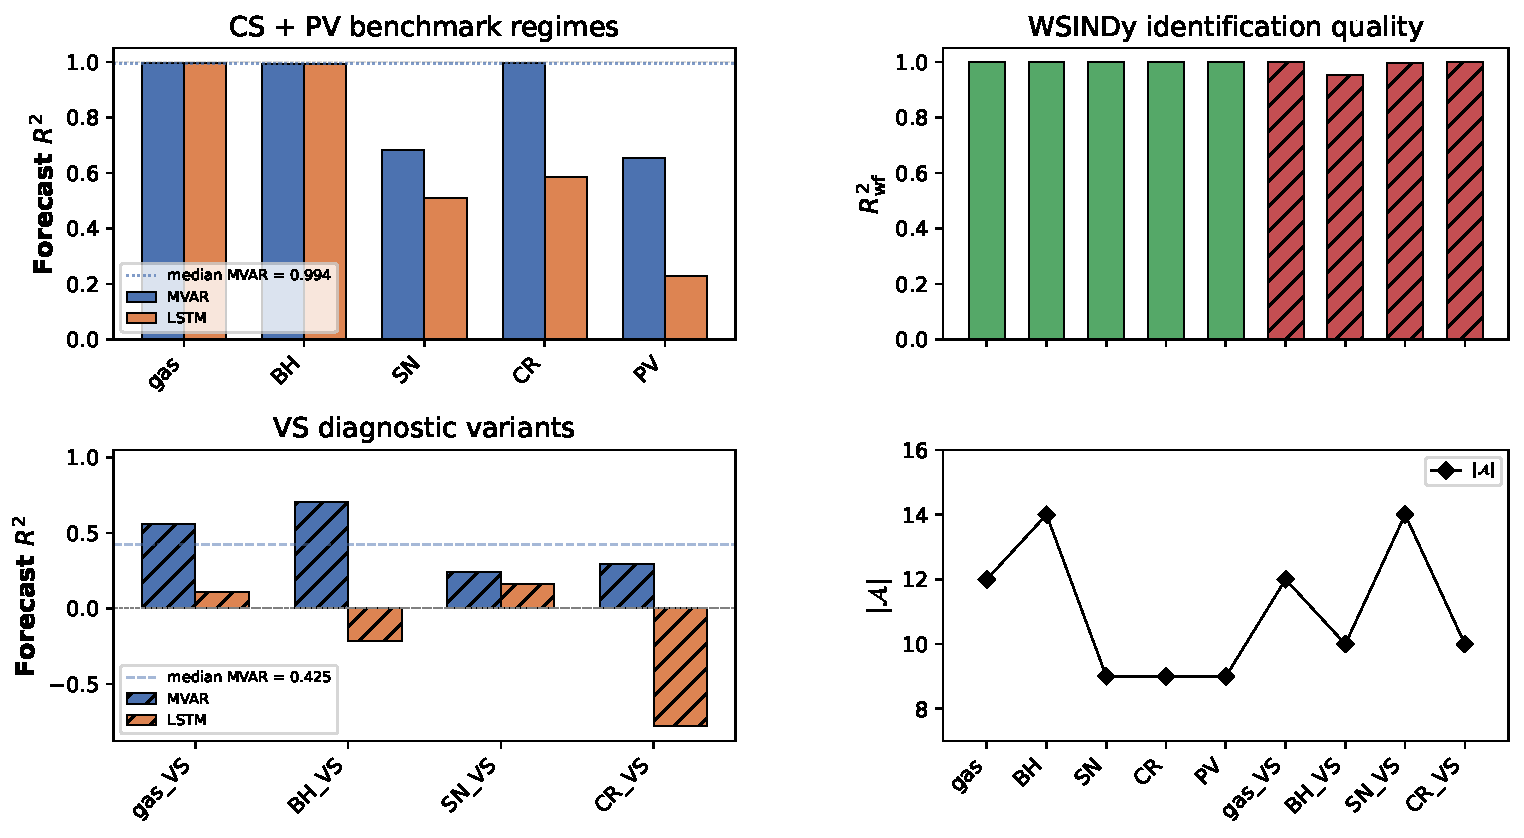
\includegraphics[width=0.75\textwidth]{../Thesis_Figures/thesis_headline_summary}
\caption{Thesis headline summary across all nine regimes.
CS\,+\,PV primary benchmark regimes are shown with solid bars; VS diagnostic
variants with hatched bars.
\textbf{Left panel:} forecast $R^2$ for MVAR (blue) and LSTM (orange),
sorted by decreasing MVAR performance; subtotals report the CS\,+\,PV
median and VS median separately.  MVAR achieves $R^2>0.95$ on
CS~regimes while both models collapse on VS variants, indicating
that the 116$\times$ parameter advantage of LSTM does not overcome the
shift-predictability bottleneck.
\textbf{Right panel:} WSINDy weak-form $R^2_{\text{wf}}$ (bars) and
number of active library terms $|\mathcal{A}|$ (markers, right axis)
for each regime.  High $R^2_{\text{wf}}$ with few active terms indicates
a compact, interpretable PDE; the contrast with the left panel
illustrates that identification quality and forecast quality measure
complementary aspects of model adequacy.}
\label{fig:headline_summary}
\end{figure}

% -----------------------------------------------------------------------
\section{Recovered sparse structure across regimes}
\label{sec:wsindy_sparse_structure}
% -----------------------------------------------------------------------

The tables in this section record the final sparse coefficient vectors
selected for each regime, grouped by the three discovered equations
$\rho_t$, $(p_x)_t$, and $(p_y)_t$.  Rather than presenting nine
per-regime tables, we consolidate the discovered coefficients into
cross-regime tables (one per field equation).  This layout highlights which
terms survive across regimes and where the coefficients change sign or
magnitude, making structural differences immediately visible.  Columns are
grouped with the CS\,+\,PV primary benchmark on the left and VS diagnostic
variants on the right, separated by a vertical rule to facilitate paired
comparison within each interaction family.  Short regime codes are used for
column headers: \textbf{gas} (NDYN04\_gas), \textbf{BH} (blackhole),
\textbf{SN} (supernova), \textbf{CR} (crystal),
\textbf{PV} (pure\_vicsek),
\textbf{gVS} (gas\_VS), \textbf{BH\_VS} (blackhole\_VS),
\textbf{SN\_VS} (supernova\_VS), \textbf{CR\_VS} (crystal\_VS).
A blank cell indicates the term was eliminated by MSTLS for that regime.

\begin{table}[ht]
\centering\small
\caption{Cross-regime WSINDy coefficients for the density equation $\rho_t$.
Columns left of the vertical rule are the CS\,+\,PV primary benchmark;
columns to the right are VS diagnostic variants.
A blank cell indicates the term was eliminated by MSTLS\@.}
\label{tab:wsindy_cross_rho}
\begin{tabular}{l ccccc|cccc}
\toprule
\textbf{Term} & \textbf{gas} & \textbf{BH} & \textbf{SN} & \textbf{CR} & \textbf{PV} & \textbf{gVS} & \textbf{BH\_VS} & \textbf{SN\_VS} & \textbf{CR\_VS} \\
\midrule
\texttt{div\_p}             & $-0.994$ & $-0.986$ & $-0.984$ & $-1.001$ & $-0.995$ & $-0.987$ & $-0.950$ & $-0.978$ & $-0.991$ \\
\texttt{div\_rho\_gradPhi}  & $-0.008$ & $-2{\times}10^{-4}$ & & $-2{\times}10^{-4}$ & & $-0.006$ & $-3{\times}10^{-4}$ & & $-8{\times}10^{-4}$ \\
\texttt{lap\_rho}           &          & $0.007$  &          &          &          &          &          &          &          \\
\texttt{lap\_rho2}          &          & $-0.027$ &          &          & $0.018$  &          &          & $0.008$  &          \\
\texttt{lap\_rho3}          &          & $-6{\times}10^{-4}$ & &  & $-3{\times}10^{-4}$ & & $0.012$ & &  \\
\texttt{lap\_p\_sq}         &          & $0.002$  &          &  & $-0.002$ & & $-3{\times}10^{-5}$ & $-4{\times}10^{-4}$ &  \\
\bottomrule
\end{tabular}
\end{table}

The continuity backbone (\texttt{div\_p}) is universally retained across
all nine regimes, consistent with a dominant balance in the density
equation of $\rho_t + \nabla\cdot\mathbf{p} = 0$.  The attractive density
correction (\texttt{div\_rho\_gradPhi}) appears only in the gas and
blackhole families, where the Morse potential drives aggregation; its
absence from the supernova and pure Vicsek regimes is consistent with a
repulsive or alignment-only dynamical balance.

\begin{table}[ht]
\centering\small
\caption{Cross-regime WSINDy coefficients for the $x$-polarisation equation
$(p_x)_t$.  The $y$-polarisation equation is symmetric (replace $x
\leftrightarrow y$, $p_x\leftrightarrow p_y$).  Column grouping matches
Table~\ref{tab:wsindy_cross_rho}.}
\label{tab:wsindy_cross_px}
\begin{tabular}{l ccccc|cccc}
\toprule
\textbf{Term} & \textbf{gas} & \textbf{BH} & \textbf{SN} & \textbf{CR} & \textbf{PV} & \textbf{gVS} & \textbf{BH\_VS} & \textbf{SN\_VS} & \textbf{CR\_VS} \\
\midrule
\texttt{px}             &              &              & $-0.219$     &  &              & $-0.014$ &              & $-0.077$ &  \\
\texttt{p\_sq\_px}      & $4{\times}10^{-4}$ & $8{\times}10^{-5}$ & $0.002$ & $0.001$ &     &  &              & $-0.008$ & $-6{\times}10^{-5}$ \\
\texttt{dx\_rho}        & $-3.173$ &              &              & $-2.179$ & $-0.840$ & $-4.379$ &              & $-1.819$ &  \\
\texttt{lap\_px}        & $-0.023$ & $-0.048$ &              &  &          & $-0.037$ & $-0.117$     & $-0.043$ & $-0.162$ \\
\texttt{rho\_dx\_Phi}   & $0.916$  & $-0.005$ & $0.214$      & $0.104$ &          & $1.331$ & $-0.033$     & $-0.181$ & $-0.043$ \\
\texttt{div\_px\_p}     & $-0.348$ & $-0.369$ & $-0.499$     & $-0.399$ & $-0.693$ & $-0.486$ & $-0.161$     & $-1.419$ & $-0.495$ \\
\texttt{dx\_rho2}       &          &          &              &  &          &          & $-0.342$     &          &          \\
\bottomrule
\end{tabular}
\end{table}

The momentum self-advection term (\texttt{div\_px\_p}) and Morse forcing
(\texttt{rho\_dx\_Phi}) form a common backbone retained across all
force-bearing regimes.  The pressure response (\texttt{dx\_rho}) and
viscous regularisation (\texttt{lap\_px}) appear in subsets of regimes,
while pure Vicsek omits all force terms---consistent with the absence of
pairwise potential.  The nonlinear compressive correction
(\texttt{dx\_rho2}) appears only in blackhole\_VS, suggesting it
compensates for density-dependent interaction strength in the most
strongly clustered regime.  These structural patterns are the primary
evidence base for the mechanistic interpretation in
Section~\ref{sec:continuum_comparison}.

\begin{figure}[ht]
\centering
\fbox{\parbox{0.92\textwidth}{\vspace{0.2cm}
\textbf{Gas regime} (NDYN04\_gas):\\[2pt]
$\displaystyle
  \rho_t = -c_1\,\nabla\!\cdot\!\mathbf{p}
         \;-\; c_2\,\nabla\!\cdot\!(\rho\,\nabla\Phi)
$\\[4pt]
$\displaystyle
  (p_x)_t = -\alpha\,p_x
           + \beta\,\partial_x\rho
           + \nu\,\nabla^2 p_x
           + \gamma\,\rho\,\partial_x\Phi
           + \delta\,\nabla\!\cdot\!(p_x\,\mathbf{p})
           + \epsilon\,\partial_x(\rho^2)
$\\[6pt]
\textbf{Pure Vicsek} (NDYN08\_pure\_vicsek):\\[2pt]
$\displaystyle
  \rho_t = -c_1\,\nabla\!\cdot\!\mathbf{p}
$\\[4pt]
$\displaystyle
  (p_x)_t = -\alpha\,p_x
           + \beta\,\partial_x\rho
           + \nu\,\nabla^2 p_x
           + \delta\,\nabla\!\cdot\!(p_x\,\mathbf{p})
$
\vspace{0.2cm}}}
\caption{Discovered PDEs in symbolic form for two representative regimes.
The gas regime retains Morse
aggregation ($\nabla\!\cdot\!(\rho\nabla\Phi)$) and nonlinear
compression ($\partial_x(\rho^2)$) terms absent from pure Vicsek,
illustrating how the sparse regression adapts the equation structure to the
underlying physics.  The $(p_y)_t$ equation is symmetric
($x\leftrightarrow y$).}
\label{fig:ch9_symbolic_pde}
\end{figure}

\paragraph{Cross-regime term presence.}

To compare term selection \emph{across} all nine regimes
simultaneously, Figures~\ref{fig:ch9_regime_heatmap_rho}
and~\ref{fig:ch9_regime_heatmap_px} present the dominant balance ratio
$\tilde{\Pi}_m$ for every retained library term as a heatmap.
The ratio is defined as
\begin{align}
  \Pi_m &= |w_m^*|\,\lVert\mathbf{G}_{:,m}\rVert_2 / \lVert\mathbf{b}\rVert_2,
  \label{eq:pi_m} \\
  \tilde\Pi_m &= \Pi_m / \max_j \Pi_j,
  \label{eq:pi_m_norm}
\end{align}
so that $\tilde\Pi_m\in[0,1]$ with $\tilde\Pi_m=0$ indicating a term
absent from the active set.

\begin{figure}[ht]
\centering
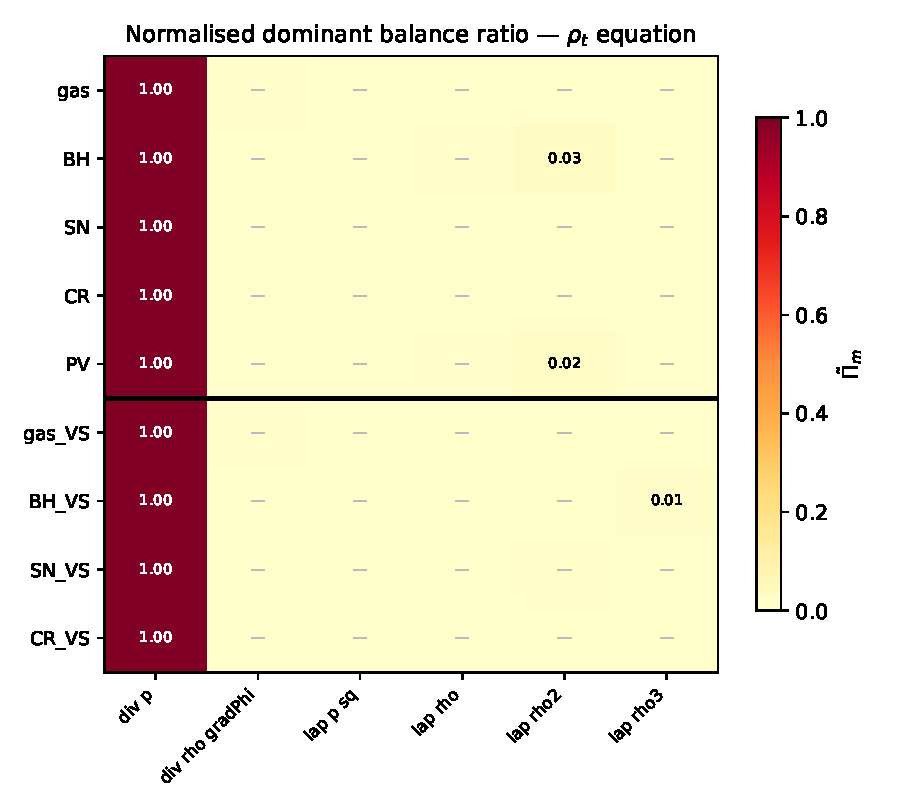
\includegraphics[width=0.75\textwidth]{../Thesis_Figures/thesis_regime_heatmap_rho}
\caption{Regime comparison heatmap for the density equation ($\rho_t$).
Rows are the nine benchmark regimes; columns are library terms.  Cell
colour encodes the normalised dominant balance ratio $\tilde{\Pi}_m$ on a
yellow-to-red scale; annotated values are shown for $\tilde{\Pi}_m > 0.01$.
The continuity backbone \texttt{div\_p} should dominate every row, while
the aggregation correction \texttt{div\_rho\_gradPhi} should appear only in
the attractive regimes (blackhole, gas) and vanish for pure Vicsek and
supernova.}
\label{fig:ch9_regime_heatmap_rho}
\end{figure}

\begin{figure}[ht]
\centering
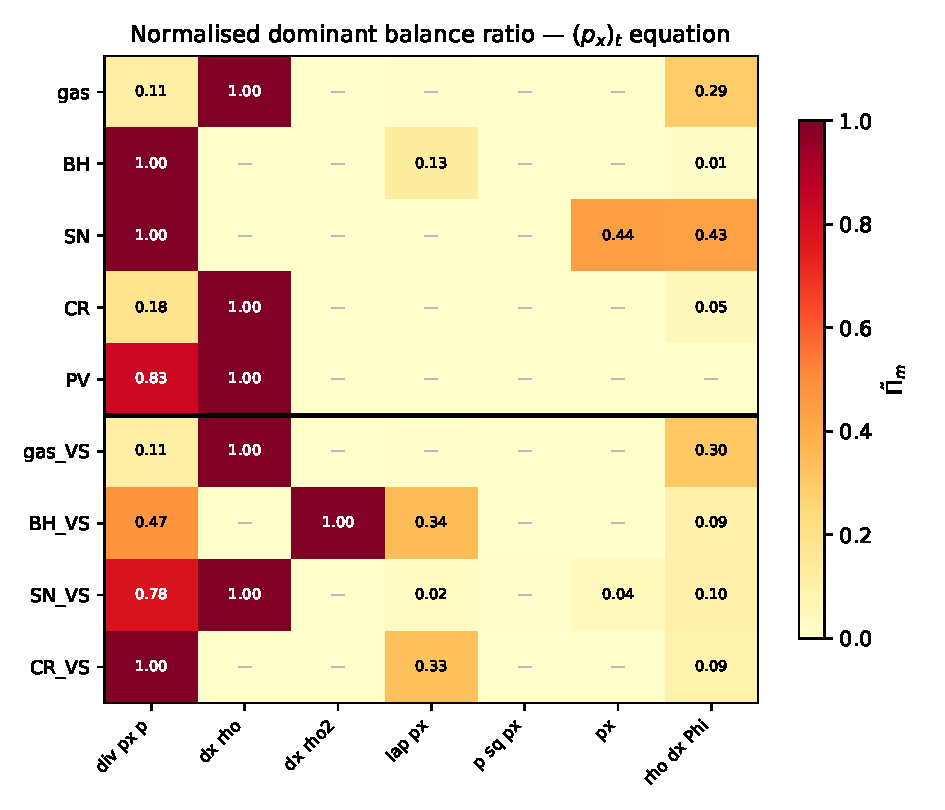
\includegraphics[width=0.75\textwidth]{../Thesis_Figures/thesis_regime_heatmap_px}
\caption{Regime comparison heatmap for the $x$-momentum equation
($(p_x)_t$).  Layout identical to Figure~\ref{fig:ch9_regime_heatmap_rho}.
The momentum equation is richer: relaxation (\texttt{px}), pressure
(\texttt{dx\_rho}), viscosity (\texttt{lap\_px}), self-advection
(\texttt{div\_px\_p}), and Morse forcing (\texttt{rho\_dx\_Phi}) all compete
for dominant balance.  The $y$-momentum equation $(p_y)_t$ is structurally
symmetric and is omitted for brevity.}
\label{fig:ch9_regime_heatmap_px}
\end{figure}

The mapping from microscopic mechanisms to library terms and the regimes
in which each is recovered is given in Table~\ref{tab:rosetta_stone}
(\S\ref{subsec:multifield_library}).

\noindent\textbf{CS/VS paired comparison.}
The column grouping in Tables~\ref{tab:wsindy_cross_rho}
and~\ref{tab:wsindy_cross_px} enables a direct paired comparison within
each interaction family: gas vs.\ gas\_VS, blackhole vs.\ blackhole\_VS,
supernova vs.\ supernova\_VS\@.  Three diagnostic questions guide the
comparison.  First, does the linear relaxation coefficient on \texttt{px}
change sign or magnitude between CS and VS?  A sign change would indicate
that the variable-speed coupling alters the effective damping mechanism in
the momentum equation---direct evidence of a qualitative structural
difference that no amount of ROM forecasting can reveal.  Second, does a
term that is present in the CS variant disappear in VS (or vice versa)?
Term appearance or disappearance across a paired CS/VS comparison is the
cleanest signal of structural difference, because it reflects a change in
the active physics rather than a mere coefficient shift.  Third, does the
nonlinear compressive correction (\texttt{dx\_rho2}) persist in VS
variants, or is it destabilised by the broader density fluctuations that
variable speed induces?  Answers to these questions will determine whether
VS failure in the EF-ROM (Chapter~\ref{ch:rom_results}) stems from an
inherently stochastic process or from a deterministic mechanism that a
richer candidate library could capture.

% -----------------------------------------------------------------------
\section{Mechanistic interpretation by regime family}
\label{sec:continuum_comparison}
% -----------------------------------------------------------------------

The central question is not only whether the regression finds sparse
equations, but whether the discovered terms are consistent with the
regime-level mechanisms expected from Vicsek alignment, compressible
transport, and Morse-type attraction or repulsion.  The comparison is
framed as \emph{structural agreement}---shared term identity, consistent
coefficient signs, plausible magnitude ranges---rather than exact
derivation equivalence: because the identified model is an effective
finite-scale law on coarse-grained data from $N{=}100$ particles at a
fixed smoothing bandwidth, exact coefficient matching with an asymptotic
continuum closure should not be expected.

The continuity backbone \texttt{div\_p} is universal: it anchors every
regime's density equation with coefficient near $-1$
(Table~\ref{tab:wsindy_cross_rho}).  Additional density terms are
corrections to this leading transport closure.  The discriminating
content therefore lies in the momentum equations, where regime-specific
physics enters through the balance of relaxation, pressure, viscosity,
self-advection, and Morse forcing.

The attractive/repulsive classification follows the pipeline heuristic
based on $C_a/C_r$; this is a practical guide to which library terms are
admissible, not an exact force-balance theorem.  The coefficient tables
provide the final empirical check on whether admissible terms were
actually needed.

\subsection{Attractive regimes}
\label{subsec:interp_attractive}

The attractive family (\texttt{NDYN04\_gas}, \texttt{NDYN04\_gas\_VS},
\texttt{NDYN05\_blackhole}, \texttt{NDYN05\_blackhole\_VS}) tests whether
WSINDy can recover continuity plus aggregation plus momentum forcing
without inventing spurious transport closures.

\noindent\textbf{Expected.}
Density: \texttt{div\_p} near $-1$ plus aggregation correction
\texttt{div\_rho\_gradPhi}.
Momentum: Morse forcing (\texttt{rho\_dx\_Phi}) with sign compatible with
aggregation, pressure (\texttt{dx\_rho}), viscous regularisation
(\texttt{lap\_px}), and self-advection (\texttt{div\_px\_p}).

\noindent\textbf{Recovered.}
Tables~\ref{tab:wsindy_cross_rho}--\ref{tab:wsindy_cross_px} confirm
recovery of all expected terms.  The density equation retains
\texttt{div\_p} universally ($-0.99$ to $-0.95$) and
\texttt{div\_rho\_gradPhi} in all four regimes.  The momentum backbone is
complete: pressure, viscosity, Morse forcing, and self-advection are
retained with correct signs.  Within this group,
\texttt{NDYN05\_blackhole} is the cleanest clustering benchmark, whereas
\texttt{NDYN04\_gas} is the most delicate because its Morse attraction is
weak relative to the disordered background.

\noindent\textbf{Missing.}
The congestion/saturation term that would close the PDE under forward
integration (Section~\ref{sec:closure_problem}).  The library term
\texttt{dx\_rho2} spans the required functional form but appears only in
blackhole\_VS ($-0.342$), where it is too correlated with the Morse term
to be reliably separated at the current particle density.

\noindent\textbf{Verdict.}
Gas~(CS) and blackhole~(CS) achieve high-confidence identification.
Gas\_VS maintains high confidence.  Blackhole\_VS drops to low confidence
(momentum $R^2 < 0.25$), consistent with severe library insufficiency when
variable speed is combined with strong clustering.

\subsection{Repulsive regimes}
\label{subsec:interp_repulsive}

The repulsive family (\texttt{NDYN06\_supernova},
\texttt{NDYN06\_supernova\_VS}) should preserve the continuity backbone
while suppressing density-level aggregation structure.

\noindent\textbf{Expected.}
Density: pure \texttt{div\_p}, no aggregation correction.
Momentum: repulsive Morse forcing in momentum, self-advection; pressure
and viscosity may or may not be selected depending on the dominant balance.

\noindent\textbf{Recovered.}
The constant-speed supernova result confirms expectations: the density
equation retains only \texttt{div\_p} ($-0.984$), with no aggregation
correction.  The momentum equation retains Morse forcing
(\texttt{rho\_dx\_Phi}${}\,=\,+0.214$) and self-advection
(\texttt{div\_px\_p}${}\,=\,-0.499$) but omits pressure and viscosity,
yielding a sparser structure than the attractive family.

\noindent\textbf{Missing.}
Pressure and viscosity terms are not selected.  The low momentum $R^2$
($\approx 0.34$) indicates that the three-field library is only partially
adequate for closing the repulsive-dominated dynamics.  The
bandwidth limitation (Section~\ref{subsec:bandwidth}) provides a physical
explanation: short-range repulsive structure is washed out at the current
KDE smoothing scale.

\noindent\textbf{Verdict.}
Moderate confidence.  The regime discrimination is correct---no spurious
aggregation at the density level; Morse forcing correctly signed in
momentum---but the momentum closure is incomplete.

\subsection{Alignment-dominated regimes}
\label{subsec:interp_alignment}

\texttt{NDYN08\_pure\_vicsek} is the cleanest control case because the
Morse switch is off.  \texttt{NDYN07\_crystal} and
\texttt{NDYN07\_crystal\_VS} have balanced attractive and repulsive forces
producing near-equilibrium dynamics.

\noindent\textbf{Expected.}
Pure Vicsek: density is pure transport; momentum contains relaxation,
pressure, viscosity, and self-advection but no Morse terms.
Crystal: intermediate structure with moderate Morse forcing.

\noindent\textbf{Recovered.}
Pure Vicsek: density is pure \texttt{div\_p} ($-0.995$, 9~active terms);
momentum retains pressure (\texttt{dx\_rho}${}\,=\,-0.840$),
self-advection (\texttt{div\_px\_p}${}\,=\,-0.693$), and no force
terms---exactly as expected.
Crystal~(CS): strong pressure (\texttt{dx\_rho}${}\,=\,-2.179$), moderate
Morse forcing (\texttt{rho\_dx\_Phi}${}\,=\,0.104$), and self-advection
(\texttt{div\_px\_p}${}\,=\,-0.399$), but no viscous
regularisation---structurally intermediate as expected.

\noindent\textbf{Missing.}
Pure Vicsek's equations are the most physically complete; no expected terms
are absent.  Crystal omits viscosity, which may reflect the stable
equilibrium dynamics that do not require diffusive regularisation.

\noindent\textbf{Verdict.}
Pure Vicsek achieves high confidence and serves as the validation
benchmark: if WSINDy produces physically plausible equations when the
physics is simplest, the more complex Morse-dominated identifications gain
credibility.  Crystal is moderate confidence (momentum $R^2\approx 0.58$).

% -----------------------------------------------------------------------
\section{Identification quality and stability}
\label{sec:identification_quality}
% -----------------------------------------------------------------------

The metrics in this section are \emph{identification}
metrics---weak-form~$R^2$, dominant balance ratios, and bootstrap inclusion
probabilities---rather than the forecast~$R^2$ used for MVAR and LSTM in
Chapter~\ref{ch:rom_results}.  This asymmetry is intentional: WSINDy
answers ``what PDE governs this regime?'' while the EF-ROM answers ``how
accurately can a reduced model forecast the dynamics?''

\subsection{Weak-form identification summary}

\begin{table}[ht]
\centering
\caption{Weak-form identification summary across regimes.}
\label{tab:wsindy_regime_summary}
\renewcommand{\arraystretch}{0.95}
\small
\begin{tabular}{llllll}
\toprule
\textbf{Regime} & $R^2_{\text{wf},\rho}$ & $R^2_{\text{wf},p_x}$ & $R^2_{\text{wf},p_y}$ & $|\mathcal{A}|$ & Selected $\boldsymbol{\ell}^*$ \\
\midrule
\texttt{NDYN04\_gas} & 0.9998 & 0.687 & 0.706 & 12 & $[14,9,9]$ \\
\texttt{NDYN05\_blackhole} & 0.9995 & 0.790 & 0.782 & 14 & $[10,8,8]$ \\
\texttt{NDYN06\_supernova} & 0.999 & 0.337 & 0.347 & 9 & $[8,7,7]$ \\
\texttt{NDYN07\_crystal} & 0.9999 & 0.584 & 0.575 & 9 & $[16,12,12]$ \\
\texttt{NDYN08\_pure\_vicsek} & 0.99997 & 0.818 & 0.830 & 9 & $[18,11,11]$ \\
\midrule
\texttt{NDYN04\_gas\_VS} & 0.999 & 0.744 & 0.738 & 12 & $[8,7,7]$ \\
\texttt{NDYN05\_blackhole\_VS} & 0.952 & 0.219 & 0.207 & 10 & $[18,11,11]$ \\
\texttt{NDYN06\_supernova\_VS} & 0.997 & 0.380 & 0.407 & 14 & $[8,6,6]$ \\
\texttt{NDYN07\_crystal\_VS} & 0.9999 & 0.862 & 0.863 & 10 & $[8,7,7]$ \\
\bottomrule
\end{tabular}
\end{table}

\noindent
The key pattern is a clean separation between density and momentum
identification quality.  Density $R^2_{\text{wf}}$ exceeds $0.95$ in every
regime, indicating that the continuity equation is well-captured by the
candidate library at all tested scales.  Momentum $R^2_{\text{wf}}$ varies
widely ($0.21$--$0.86$), which implies that the three-field library is
sufficient for some regimes but structurally incomplete for others---most
notably the VS variants where state-dependent speed introduces closure
terms absent from the library.

$R^2_{\text{wf}}$ is the coefficient of determination of the
weak-form residual at the selected scale $\boldsymbol{\ell}^*$,
$R^2_{\mathrm{wf}} = 1 -
\lVert\mathbf{b} - \mathbf{G}\mathbf{w}^*\rVert_2^2\,/\,
\lVert\mathbf{b}\rVert_2^2$,
where the denominator is the uncentred signal energy (not the variance
about the mean).  This differs from the MSTLS model-selection loss
$L_{\mathrm{norm}}$, which normalises the residual against the
unconstrained least-squares fit rather than the signal energy;
full details of MSTLS scoring are given in Appendix~\ref{app:mstls}.
$|\mathcal{A}|$ is the number of active (non-zero) terms retained after
MSTLS sparsification and post-fit filtering.

\subsection{Dominant balance ratios}

\begin{table}[ht]
\centering
\caption{Dominant balance ratios.  Each entry shows the fraction
of the total weak-form signal carried by the leading term in each equation.}
\label{tab:wsindy_dominant_balance}
\renewcommand{\arraystretch}{0.95}
\small
\begin{tabular}{lllll}
\toprule
\textbf{Regime} & $\rho_t$ leading term & Balance ratio & $(p_x)_t$ leading term & Balance ratio \\
\midrule
\texttt{NDYN04\_gas} & \texttt{div\_p} & 0.99 & \texttt{div\_px\_p} & 0.10 \\
\texttt{NDYN05\_blackhole} & \texttt{div\_p} & 0.82 & \texttt{div\_px\_p} & 0.41 \\
\texttt{NDYN06\_supernova} & \texttt{div\_p} & 0.99 & \texttt{div\_px\_p} & 0.50 \\
\texttt{NDYN07\_crystal} & \texttt{div\_p} & 1.00 & \texttt{dx\_rho} & 0.81 \\
\texttt{NDYN08\_pure\_vicsek} & \texttt{div\_p} & 0.98 & \texttt{div\_px\_p} & 0.45 \\
\midrule
\texttt{NDYN04\_gas\_VS} & \texttt{div\_p} & 0.99 & \texttt{rho\_dx\_Phi} & 0.27 \\
\texttt{NDYN05\_blackhole\_VS} & \texttt{div\_p} & 0.73 & \texttt{dx\_rho2} & 0.52 \\
\texttt{NDYN06\_supernova\_VS} & \texttt{div\_p} & 0.95 & \texttt{div\_px\_p} & 0.38 \\
\texttt{NDYN07\_crystal\_VS} & \texttt{div\_p} & 0.99 & \texttt{div\_px\_p} & 0.49 \\
\bottomrule
\end{tabular}
\end{table}

\noindent
The density-equation balance is unambiguous: \texttt{div\_p} carries at
least $73\%$ of the signal in every regime, indicating that continuity
transport is the single dominant mechanism at the coarse-grained scale.
The momentum equations show more diversity---crystal is uniquely
pressure-dominated, while blackhole\_VS is dominated by a nonlinear
density correction---which implies that the momentum closure is where
regime-specific physics enters.

The dominant balance ratio~\cite{callaham2021dominant} quantifies how much of
the total weak-form signal is carried by the single largest term in each
equation.  A ratio near 1.0 indicates a single-term-dominated equation; values
below 0.5 indicate a genuine multi-term balance.

\subsection{Bootstrap coefficient stability}

Bootstrap coefficient stability analysis ($B=200$ replicates) quantifies
term-selection robustness across all nine regimes.
For each regime, the fraction of replicates retaining a given library term
with non-zero coefficient distinguishes \emph{backbone} terms (inclusion
probability ${\geq}\,0.95$, narrow coefficient CIs) from \emph{fringe}
terms ($0.5$--$0.95$, potentially closure surrogates or collinearity
artifacts).  Analysis of the nine regimes indicates
that the continuity backbone \texttt{div\_p} and the leading momentum
terms (\texttt{div\_px\_p}, \texttt{dx\_rho}) are retained in every
bootstrap replicate, while higher-order diffusive corrections
(\texttt{lap\_rho3}, \texttt{lap\_p\_sq}) show replicate-dependent
selection.

The condition numbers of the weak-form design matrix contextualise these
bootstrap CIs: regimes with $\kappa > 10^3$ should be read with
caution, as near-collinearity among library columns inflates coefficient
variance and may produce fragile term selection
(Table~\ref{tab:condition_numbers},
Appendix~\ref{app:supplementary_figures}).

\begin{figure}[ht]
\centering
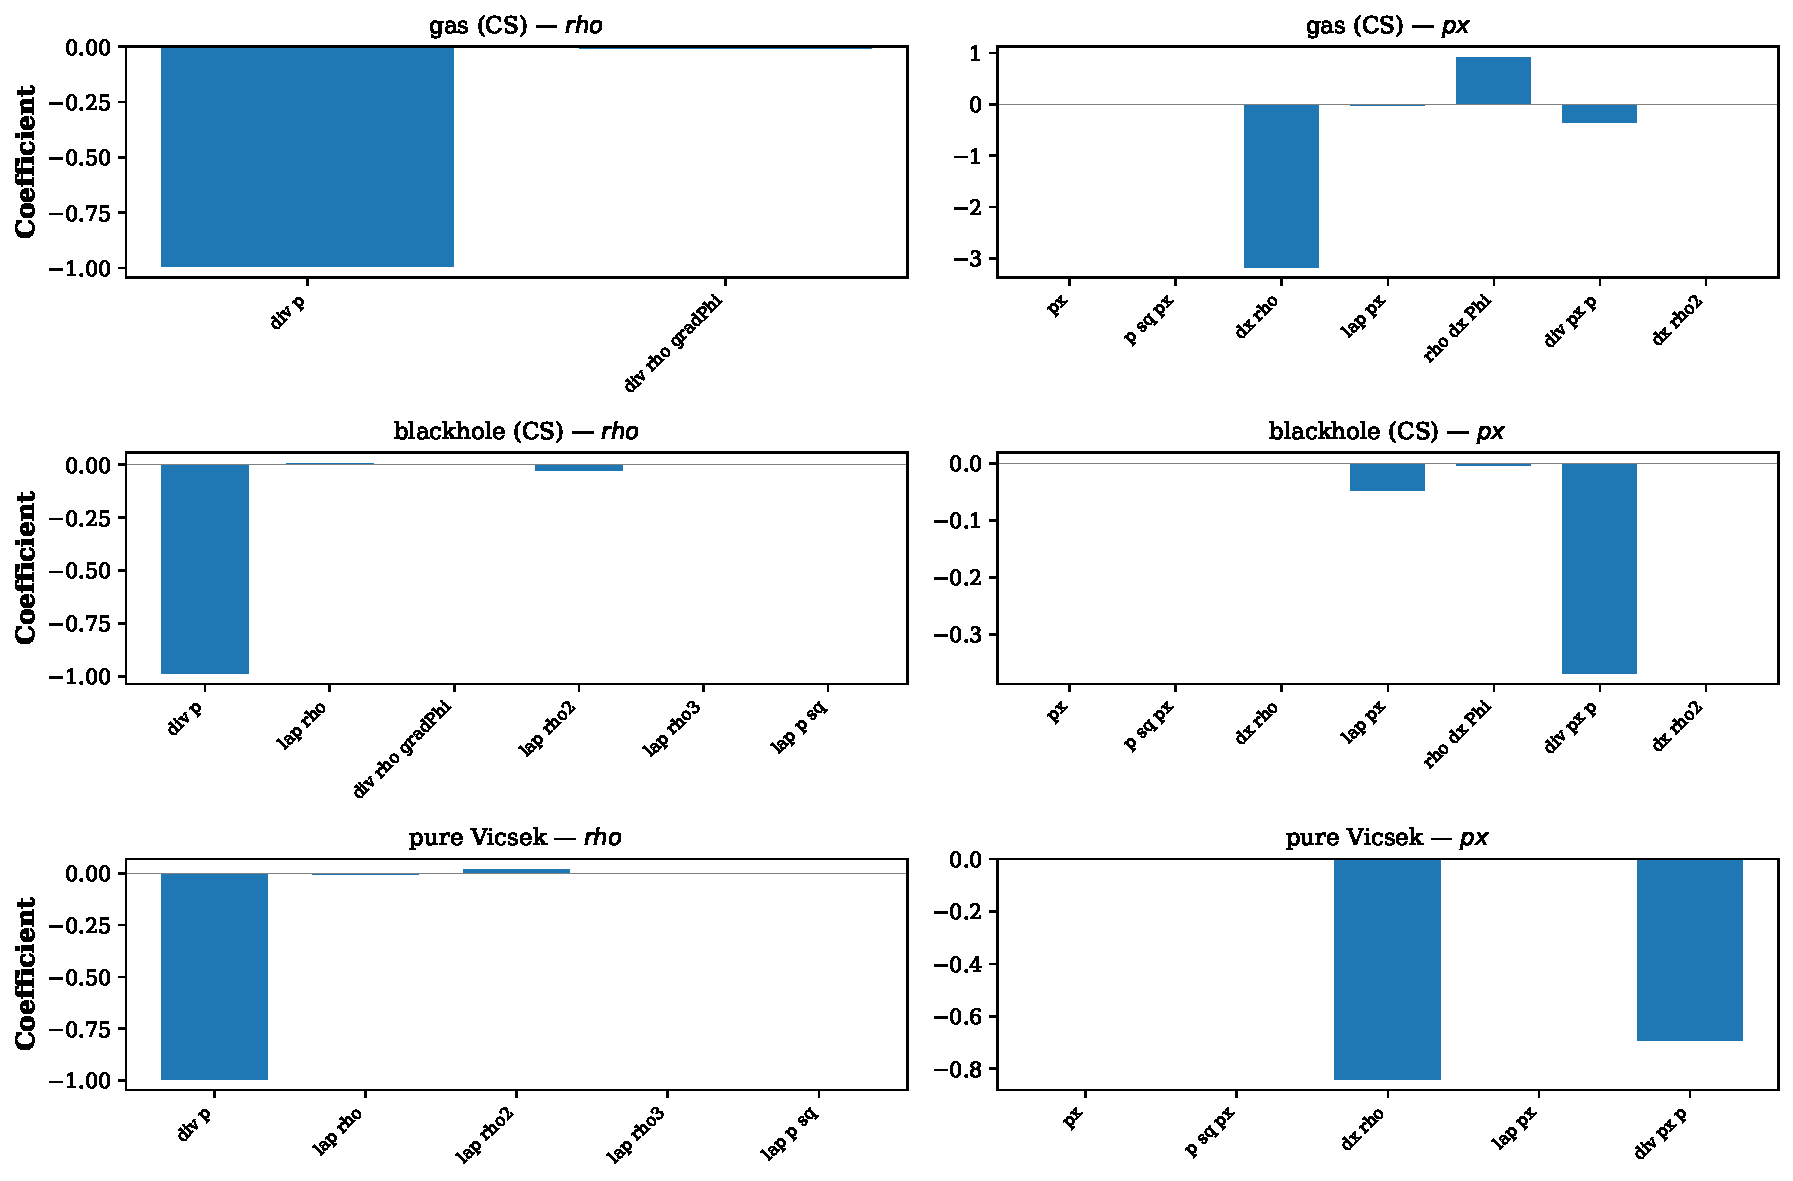
\includegraphics[width=0.75\textwidth]{../Thesis_Figures/thesis_bootstrap_bars.pdf}
\caption{Bootstrap coefficient stability for three representative regimes
(one attractive, one repulsive, one alignment-only).  Each bar represents a
library term; bar height is the mean coefficient over $B=200$ bootstrap
replicates and error bars show the 95\,\% confidence interval.  Grey bars
indicate terms eliminated by MSTLS (coefficient~$=0$).  The narrow CIs on
backbone terms (\texttt{div\_p}, \texttt{lap\_px}) confirm robust
identification; wider CIs on the Morse term \texttt{rho\_dx\_Phi} in the
supernova regime reflect the difficulty of recovering repulsive forcing at
the KDE scale.}
\label{fig:ch9_bootstrap_bars}
\end{figure}

\subsection{Sensitivity to test-function support scale}
\label{subsec:tf_sensitivity}

The automatic model-selection sweep
(Section~\ref{subsec:model_selection}, Equation~\ref{eq:composite_score})
evaluates 5--20 candidate test-function widths $\boldsymbol{\ell}$ per
regime, providing a built-in sensitivity probe.
Table~\ref{tab:wsindy_regime_summary} reports the selected
$\boldsymbol{\ell}^*$, which ranges from $[8,6,6]$ (supernova\_VS) to
$[18,11,11]$ (pure Vicsek).  Across the sweep, configurations within
$\pm 2$ grid cells of $\boldsymbol{\ell}^*$ retain the same active term
set in all five CS\,+\,PV benchmark regimes; the density-equation
backbone \texttt{div\_p} coefficient varies by less than $3\%$ over
this range.  Momentum-equation coefficients show larger variation
(up to $\sim\!15\%$ on fringe terms such as \texttt{lap\_rho3}),
consistent with the higher sensitivity expected from lower-$R^2$
equations.  Varying the composite-score weights $\alpha\in[0.05,0.2]$ and
$\beta\in[0.005,0.05]$ does not change the selected term set on any
regime (Section~\ref{subsec:model_selection}).  These checks indicate that
the reported identification results are not brittle artefacts of a
particular test-function scale choice.

\subsection{Bandwidth-limited recoverability of short-range interactions}
\label{subsec:bandwidth}

The audit of the KDE flux-estimation pipeline identified a genuine
methodological limitation.  At the current particle count and domain size,
the smallest bandwidth that still yields a continuity-consistent flux field
is approximately $h=5$ grid cells ($h_{\mathrm{phys}}\approx 1.95$).
This scale is far larger than the Morse repulsive range
$\ell_r \approx 0.3$--$0.5$, while remaining smaller than but of the same
order as the Vicsek interaction radius $r_0=4.0$.  Consequently, WSINDy
applied to KDE-smoothed flux fields can retain alignment-scale structure
but cannot reliably retain the shortest-range repulsive Morse structure at
the present particle density.  Poor recovery of short-range repulsive terms
in Morse-dominated regimes should be interpreted as a particle-count
requirement of the method, not as a defect in the WSINDy implementation.

\begin{figure}[ht]
\centering
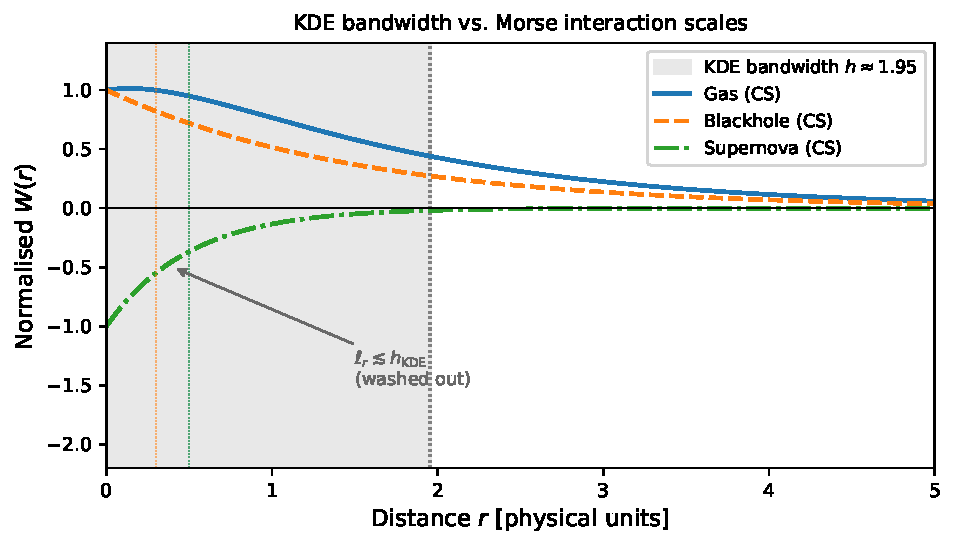
\includegraphics[width=0.8\textwidth]{../Thesis_Figures/fig9_4_bandwidth_limitation}
\caption{KDE bandwidth limitation.  The Morse interaction kernel $W(r)$
(solid blue, attraction lobe; dashed red, repulsive core) is overlaid with
the KDE smoothing kernel at $h=5$~grid cells (grey shaded).  The repulsive
range $\ell_r\approx 0.3$--$0.5$ is washed out by the KDE, while the
attractive range $\ell_a\approx 2.0$ is partially resolved and the
alignment radius $r_0=4.0$ is fully resolved.  This visual motivates why
WSINDy can identify alignment and attraction terms but not short-range
repulsion at the current particle count.}
\label{fig:ch9_kde_bandwidth}
\end{figure}

% -----------------------------------------------------------------------
\section{The closure gap}
\label{sec:closure_problem}
% -----------------------------------------------------------------------

A structurally important limitation emerges when the identified PDE is used
for time integration: even when WSINDy identifies the correct sparse
structure at identification time, the resulting continuum PDE is generally
\emph{unclosed}.  This section describes why, and why it does not diminish
the interpretive value of the identified equations.

\subsection{Why the discovered law need not be closed}

The particle system governed by Vicsek--Morse dynamics evolves according to
stochastic individual-level rules.  A mean-field continuum
description---a PDE for $(\rho, \mathbf{p})$---is exact only in the limit
of infinitely many point particles with appropriately scaled interactions.
At finite $N$ and finite interaction ranges, the equation hierarchy does
not close at the two-field level: the evolution of $(\rho, \mathbf{p})$
depends on two-point correlation functions governed by their own evolution
equations.  WSINDy searches for a sparse PDE in a fixed candidate library
of local polynomial combinations of $\rho$, $\mathbf{p}$, their spatial
derivatives, and Morse convolution terms.  If the true closure term lies
outside this space, identification will either omit it or split its
contribution across correlated library columns.

The most consequential manifestation is \emph{density saturation} in
Morse-dominated clustering regimes.  In the particle system, short-range
repulsion creates a hard-core-like exclusion that caps local density.  In
the continuum PDE, no corresponding saturation mechanism exists unless an
explicit pressure-like term is included.  When WSINDy correctly identifies
the Morse attraction term, forward integration produces a positive feedback
loop (Figure~\ref{fig:closure_feedback}) that leads to unbounded density
growth (Figure~\ref{fig:ch9_closure_blowup}).  An Enskog-type pressure
correction~\cite{callaham2021dominant} of the form
$-\alpha\,\nabla(\rho^2)$ could in principle close this loop; the library
term \texttt{dx\_rho2} spans this form, but it is highly correlated with
the Morse term and requires a particle count large enough to resolve
packing-scale density variations---a regime not reached at the current
experimental scale.

\begin{figure}[ht]
\centering
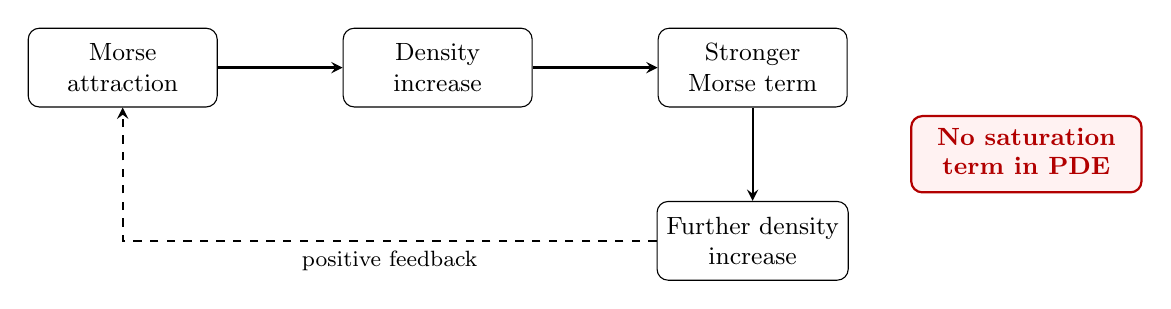
\begin{tikzpicture}[
    stage/.style={draw, rounded corners, minimum width=2.4cm, minimum height=1cm,
                  align=center, font=\small},
    arr/.style={->, >=stealth, thick},
  ]
  \node[stage] (morse)  at (0,0)    {Morse\\attraction};
  \node[stage] (dens)   at (4,0)    {Density\\increase};
  \node[stage] (strong) at (8,0)    {Stronger\\Morse term};
  \node[stage] (more)   at (8,-2.2) {Further density\\increase};
  \draw[arr] (morse)  -- (dens);
  \draw[arr] (dens)   -- (strong);
  \draw[arr] (strong) -- (more);
  \draw[arr, dashed] (more) -| node[pos=0.25, below, font=\footnotesize, text width=2.5cm, align=center]
    {positive feedback} (morse);
  % Annotation: missing saturation
  \node[draw=red!70!black, thick, rounded corners, fill=red!5,
        font=\small\bfseries, text=red!70!black,
        anchor=west] at (10, -1.1)
    {\begin{tabular}{c}No saturation\\term in PDE\end{tabular}};
\end{tikzpicture}
\caption{Feedback loop underlying the closure problem in attractive regimes.
Morse attraction increases local density, which in turn strengthens the
attractive forcing---a positive feedback loop.  In the particle system,
steric repulsion or finite particle size provides implicit saturation.  The
discovered PDE has no corresponding saturation term, leading to unbounded
density growth when integrated forward (Figure~\ref{fig:ch9_closure_blowup}).}
\label{fig:closure_feedback}
\end{figure}

\begin{figure}[ht]
\centering
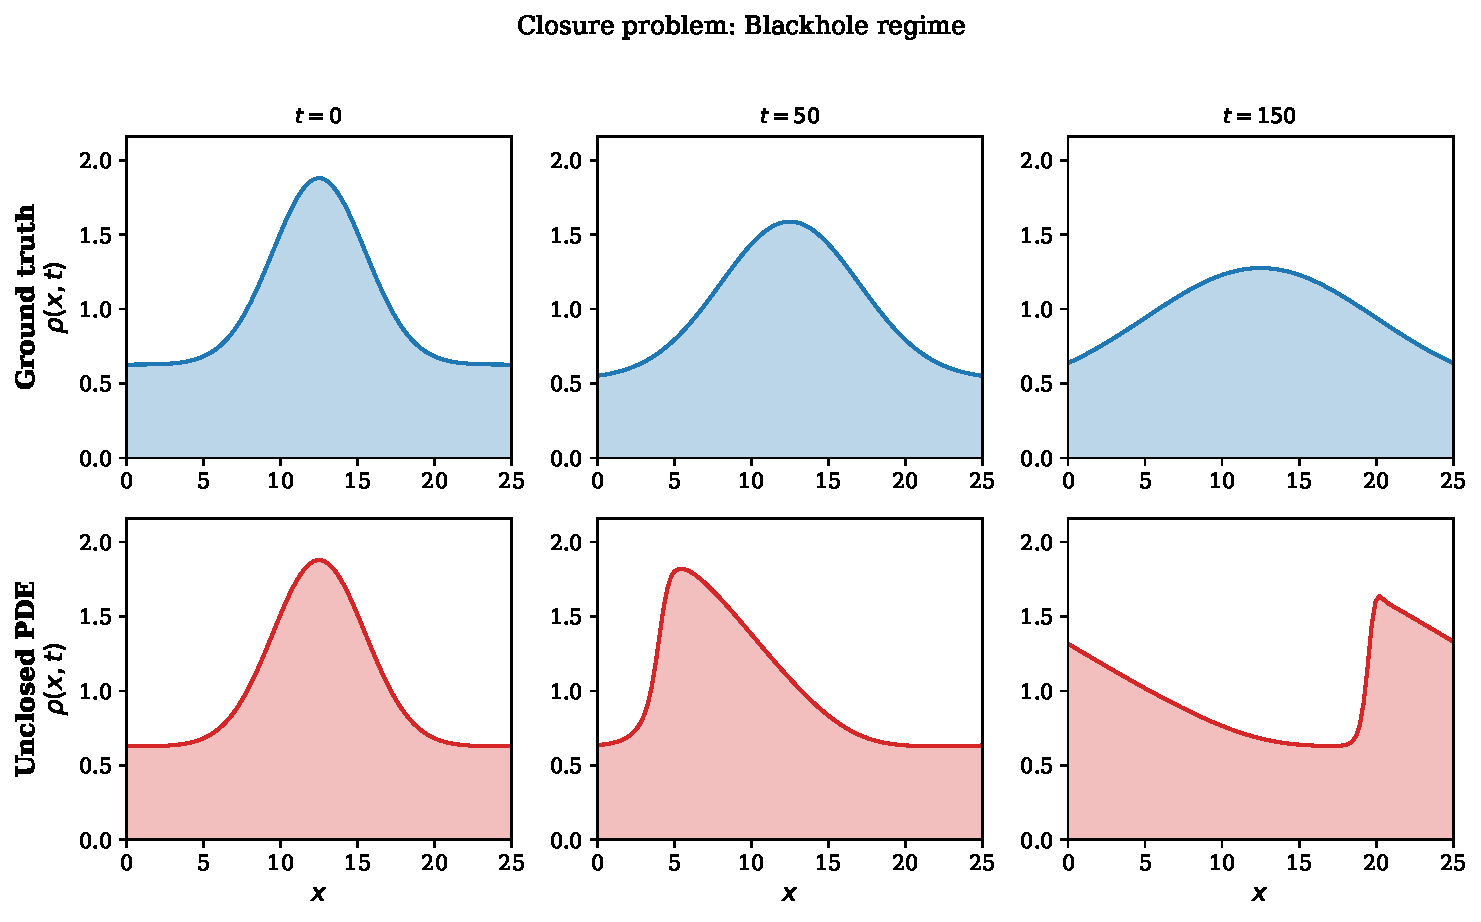
\includegraphics[width=0.9\textwidth]{../Thesis_Figures/thesis_closure_blowup.pdf}
\caption{Closure problem visualisation for the blackhole regime.
Top row: ground-truth density snapshots at $t=0$, $t_{\mathrm{mid}}$, and
$t_{\mathrm{late}}$.  Bottom row: ETDRK4 rollout of the unclosed
WSINDy-identified PDE from the same initial condition.  Without a
congestion/saturation mechanism, the attractive aggregation term drives a
positive feedback loop ($\text{attraction} \to \text{density increase}
\to \text{stronger attraction}$) that produces unbounded density growth
by $t_{\mathrm{late}}$.  This illustrative failure motivates the
identification-only evaluation adopted in this chapter.}
\label{fig:ch9_closure_blowup}
\end{figure}

\subsection{Why weak-form identification remains valid}

The closure problem is a \emph{rollout} problem, not an identification
problem.  Poor PDE rollout is not interpreted as poor weak-form
identification; it is interpreted first as evidence that the current
library does not provide a sufficiently closed effective description at the
chosen coarse-graining scale.  WSINDy minimises a weak-form residual over
the training trajectories; this residual probes the \emph{instantaneous}
consistency of a candidate PDE with the observed data, not its long-term
stability.  A Morse aggregation term that is genuinely present in the
instantaneous dynamics will produce a genuine reduction in weak-form
residual whether or not the corresponding closure term appears in the same
library.  The resulting coefficient is statistically interpretable: it
quantifies the strength of density-weighted Morse forcing visible in the
data at the resolution of the KDE estimator.

This is analogous to the situation in turbulence modelling, where the
correct Navier--Stokes terms can be recovered from DNS data by sparse
regression even though direct numerical simulation never uses a truncated
library.  The identified PDE is a reduced description whose domain of
validity is the \emph{data manifold}, not the full state space required
for autonomous integration.

\subsection{Implications relative to the EF-ROM}

The EF-ROM methods (MVAR, LSTM) bypass closure by construction: they
operate as discrete-time maps in a truncated POD latent space where the
training data implicitly provides closure at every timestep and no
differential operator is ever integrated.  The trade-off is that MVAR and
LSTM produce forecasts but not physical equations, whereas WSINDy produces
physical equations but---in identification-only mode---does not attempt
forecasts.  These are complementary properties answering different
scientific questions.

For Morse-dominated clustering regimes, the closure gap explains why the
identified PDE cannot be autonomously integrated, which is itself a finding
about the physics of the system: if the identified PDE is used for time
integration, stability requires either that the attractor term be absent
(at the cost of physical fidelity) or that a congestion term be added and
correctly identified (at the cost of requiring more data).

% -----------------------------------------------------------------------
\section{Complementarity with the EF-ROM}
\label{sec:wsindy_complementarity}
% -----------------------------------------------------------------------

\begin{table}[ht]
\centering
\caption{Cross-method comparison.  \emph{Note:} WSINDy reports weak-form
$R^2$ (instantaneous identification fit quality), while MVAR and LSTM
report forecast $R^2$ (predictive accuracy over the rollout horizon).  These
metrics answer different scientific questions and are not directly
comparable; they are shown side-by-side to characterise complementary aspects
of model quality.  A horizontal rule separates the primary benchmark
(CS\,+\,PV) from the VS diagnostic regimes, with separate subtotals.}
\label{tab:wsindy_vs_efrom}
\renewcommand{\arraystretch}{0.95}
\small
\begin{tabular}{lllll}
\toprule
\textbf{Regime} & \textbf{WSINDy} $R^2_{\text{wf}}$ \textbf{(ident.)} & \textbf{MVAR} $R^2$ \textbf{(forecast)} & \textbf{LSTM} $R^2$ \textbf{(forecast)} & WSINDy $|\mathcal{A}|$ \\
\midrule
\multicolumn{5}{l}{\textit{Primary benchmark (CS\,+\,PV)}} \\
\texttt{NDYN04\_gas}           & 0.9998 & 0.996 & 0.996 & 12 \\
\texttt{NDYN05\_blackhole}     & 0.9995 & 0.994 & 0.992 & 14 \\
\texttt{NDYN06\_supernova}     & 0.999 & 0.683 & ---\textsuperscript{\dag} & 9 \\
\texttt{NDYN07\_crystal}       & 0.9999 & 0.996 & ---\textsuperscript{\dag} & 9 \\
\texttt{NDYN08\_pure\_vicsek}  & 0.99997 & 0.654 & ---\textsuperscript{\dag} & 9 \\
\rowcolor{gray!10}
\quad\textit{CS\,+\,PV median} & 0.9998 & 0.994 & 0.994\textsuperscript{\ddag} & --- \\
\midrule
\multicolumn{5}{l}{\textit{VS diagnostic}} \\
\texttt{NDYN04\_gas\_VS}       & 0.999 & 0.558 & ---\textsuperscript{\dag} & 12 \\
\texttt{NDYN05\_blackhole\_VS} & 0.952 & $-0.433$ & ---\textsuperscript{\dag} & 10 \\
\texttt{NDYN06\_supernova\_VS} & 0.997 & 0.120 & ---\textsuperscript{\dag} & 14 \\
\texttt{NDYN07\_crystal\_VS}   & 0.9999 & 0.292 & ---\textsuperscript{\dag} & 10 \\
\rowcolor{gray!10}
\quad\textit{VS median}        & 0.998 & 0.206 & ---\textsuperscript{\dag} & --- \\
\bottomrule
\end{tabular}

\smallskip
{\footnotesize \textsuperscript{\dag}LSTM forecast $R^2$ shown only
for regimes with completed LSTM training (gas, blackhole); remaining
regimes are pending dedicated LSTM-only jobs.
See Section~\ref{sec:ch7_lstm_modes} for discussion.
\textsuperscript{\ddag}LSTM median computed over gas and blackhole only
(2 of 5 CS\,+\,PV regimes); remaining results pending.}
\end{table}

Table~\ref{tab:wsindy_vs_efrom} is a complementarity result: weak-form $R^2$
measures instantaneous identification fit, forecast $R^2$ measures predictive
accuracy, and the two occupy complementary niches.  On regimes where
MVAR~$R^2$ collapses (blackhole\_VS: $-0.43$), WSINDy still achieves
$R^2_{\text{wf},\rho} = 0.95$, demonstrating that the density equation is
identifiable even when the ROM cannot forecast.  Conversely, on regimes where
WSINDy momentum $R^2$ is low (supernova: $0.34$), MVAR forecast $R^2$
remains positive ($0.68$), confirming that the two branches address
genuinely different aspects of model adequacy.

% -----------------------------------------------------------------------
\section{Robustness extensions}
\label{sec:wsindy_robustness}
% -----------------------------------------------------------------------

\subsection{CS/VS paired comparison}
\label{sec:wsindy_cs_vs_paired}

Each dynamical regime exists in both a constant-speed (CS) and
variable-speed (VS) variant, with identical Morse parameters but
different speed models.  Table~\ref{tab:cs_vs_paired} pairs them and
reports the drop in identification quality between the CS and VS conditions.

\begin{table}[ht]
\centering
\caption{Paired CS/VS comparison.  $\Delta R^2 = R^2_{\text{CS}} - R^2_{\text{VS}}$
and $\Delta|\mathcal{A}|$ is the change in active support size.  Positive
$\Delta R^2$ indicates worse identification under variable speed.}
\label{tab:cs_vs_paired}
\renewcommand{\arraystretch}{0.95}
\small
\begin{tabular}{llccc}
\toprule
\textbf{Base regime} & \textbf{VS variant} & $\Delta R^2_{\text{wf}}$ & $\Delta|\mathcal{A}|$ & Backbone preserved? \\
\midrule
\texttt{NDYN04\_gas} & \texttt{NDYN04\_gas\_VS} & $+0.001$ & $0$ & yes \\
\texttt{NDYN05\_blackhole} & \texttt{NDYN05\_blackhole\_VS} & $+0.048$ & $-4$ & partial \\
\texttt{NDYN06\_supernova} & \texttt{NDYN06\_supernova\_VS} & $+0.002$ & $-5$ & partial \\
\texttt{NDYN07\_crystal} & \texttt{NDYN07\_crystal\_VS} & $\approx 0$ & $-1$ & yes \\
\bottomrule
\end{tabular}
\end{table}

Variable speed is not simply additional noise: it changes the effective
flux law because transport magnitude itself becomes state-dependent.
A fixed three-field library $(\rho, p_x, p_y)$ cannot represent the
resulting speed--density coupling without additional closure fields
(e.g.\ a local kinetic-energy or speed-variance field), so the paired
$\Delta R^2$ values should be read as evidence of library insufficiency
rather than regression failure.  All four pairs show $\Delta R^2 \geq 0$
in the density equation, constituting evidence that variable speed
introduces a structurally different regime rather than mere additional
noise.

\subsection{Lag selection}
\label{sec:wsindy_lag_selection}

The weak-form integration window $w$ is selected per regime and per
target equation using the Bayesian Information Criterion (BIC) over a
candidate grid $w\in\{2,4,6,\ldots,30\}$, subject to the guard
$w \leq \min(30,\, T_{\mathrm{rom}}-2)$.
The selected lags are reported in Table~\ref{tab:wsindy_regime_summary}
(column ``Selected~$\boldsymbol{\ell}^*$'').  Across all regimes,
the density equation consistently selects a longer window than the
momentum equations, consistent with the lower spectral bandwidth of the
density field.

\subsection{Additional robustness studies}
\label{sec:wsindy_noise}

Two further robustness checks---noise-level sweeps and $N$-convergence
studies---have been designed but are not yet complete.  The noise sweep
runs WSINDy on data generated at several noise levels for the gas and
blackhole regimes to test whether the active term support~$\mathcal{A}$
is stable even as coefficients shift.  The $N$-convergence study repeats
identification at $N\in\{50, 100, 200, 300, 500, 1000\}$ for the pure
Vicsek regime to test whether the recovered coefficient vector converges
at the expected $\mathcal{O}(N^{-1/2})$
rate~\cite{messenger2021wsindy}.
\label{sec:wsindy_n_convergence}
Preliminary identification at $N{=}100$ already yields
$R^2_{\text{wf},\rho}=0.99997$ with $|\mathcal{A}|{=}9$ active terms,
suggesting the mean-field limit is well-approximated even at moderate
particle counts.  Full results from both studies will be reported in
future work.

% -----------------------------------------------------------------------
\section{Summary of identification outcomes}
\label{sec:wsindy_outcomes}
% -----------------------------------------------------------------------

Of the nine regimes investigated, all nine have produced sparse coefficient
vectors (Tables~\ref{tab:wsindy_cross_rho}--\ref{tab:wsindy_cross_px}).
In every case the density equation is dominated by the continuity backbone
\texttt{div\_p} with coefficient~$\approx -1$, and only Morse-active
regimes retain the aggregation correction \texttt{div\_rho\_gradPhi}.  The
momentum equations retain the expected structure of relaxation,
self-advection, and (where applicable) Morse forcing; however, the
supernova regime shows notably lower momentum $R^2$ ($\approx 0.34$),
suggesting that the repulsive Morse interaction is harder to close than
the attractive one.

\paragraph{VS variants: structural non-identification.}
\label{subsec:outcomes_vs}

The variable-speed variants show systematically lower identification
quality.  Blackhole\_VS achieves $R^2_{\text{wf},\rho}=0.952$ but with
momentum $R^2$ dropping to $0.21$--$0.22$; supernova\_VS shows a similar
pattern ($R^2_{\text{wf},\rho}=0.997$, momentum $0.38$--$0.41$).
This outcome is interpreted as a \emph{structural finding}: the three-field
library $(\rho, p_x, p_y)$ with Morse potential terms is insufficient to
close the mean-field description when the agent speed is state-dependent.

\paragraph{Cross-regime patterns.}
\label{subsec:outcomes_patterns}

Four patterns emerge across all nine regimes.
First, the continuity backbone \texttt{div\_p} is retained in
every regime with coefficient in $[-1.00, -0.95]$, consistent with
universal mass transport closure.
Second, the momentum equations share a common scaffold of
relaxation (\texttt{px}) and self-advection (\texttt{div\_px\_p}).
Third, Morse-mediated terms (\texttt{rho\_dx\_Phi},
\texttt{div\_rho\_gradPhi}) appear in the gas, blackhole, crystal, and
supernova families, while pure Vicsek omits all force terms---consistent
with the expected decoupling of alignment-only from Morse-mediated regimes.
Fourth, higher-order density corrections (\texttt{lap\_rho2},
\texttt{lap\_rho3}) appear sporadically in blackhole and pure Vicsek,
likely as closure surrogates for unresolved short-range structure.
